\section{Vježba 2: Metoda podudaranja susjedstva piksela s modelom}

\subsection{Opis vježbe}
Učitati zadanu sliku na kojoj piše neki tekst. Mišem označiti
(kvadratićem zaokružiti) jedno slovo u tekstu na slici. Primjenom metode
podudaranja susjedstva piksela s modelom (engl. \textit{Template
Matching} potrebno je odrediti i označiti (kvadratićem zaokružiti) sva
slična (\textbf{ista}) slova poput označenog slova.

\subsection{Objašnjenje programa}

\subsubsection{Kontrola programa}

Prilikom pokretanja programa iz komandne linije potrebno je 
predati programu putanju do slike (argv[1]) u protivnom se program 
nece pokrenuti. \\

\begin{lstlisting}[language=bash,caption={Pokretanje programa iz
    komandne linije}]
$ ./template_matching ../images/tm-quick.png
\end{lstlisting}

Nakon pokretanja programa u ispisu komandne linije stoji da odaberemo
``t'' za pokretnje template matching-a. Međutim prije toga je prvo
potrebno odredit model odabirom slova ``r'' te nakon toga. Sada možemo
pritisnut ``t'' te će program izbaciti rezultate podudaranja susjedstva
piksel s modelom te označiti slične modele.
\\

\begin{lstlisting}[language=C,caption={Kontrola programa tipkovnicom}]
while (1){
    char c = waitKey(10);
    switch(c) {
        case 'r':
            cout << "Setting callback, calling cropImage  ...\n";
            setMouseCallback(imageName, onMouse, (void*)&loaded_img);
            break;
        case 't':
            if(!croped_roi.data){
                cout << "nisi cropao nista" << endl;
                break; }
            matchTemplateTrackbar( );
            break;
            } }
\end{lstlisting}

\subsubsection{Metoda podudaranje susjedstva piksela s modelom}
Kao što samo ime metode kaže uspoređuje se matrica modela \textbf{T}
(engl. \textit{template}) s matricom slike \textbf{I} na način da
model klizi preko slike. Nad svakim pikselom iz modela izvodi se
matematička funkcija. Funkcija vraća sličnost modela i uspoređenog
dijela slike. Tu vrijednost funkcija zapisuje u rezultantn matricu
\textbf{R}. Opisanu radnju izvršavamo pozivom funkcije
\textit{cv::matchTemplate()}. U toj funkciji je impelementirano šest
matematičkih metoda za pronalazak sličnosti. Svaku od njih se može
isprobati pomicanjem klizača. Nakon dobivanja rezultantne matrice
slijedi pronalazak pozicija piksela koji imaju najveću sličnost modela i
slike. To se možemo odraditi na više načina. Primjerice možemo korisitit 
funkciju \textit{cv::minMaxLoc()}. Ona nam vrati poziciju piksela s najvećom i
najmanjom vrijdnosti. Ta metoda je ograničena na vraćanje samo jednog 
sličnog rezultata. Drugi način je da nad normaliziranom rezultatnom
matricom (vrijdnosti prikazna brojevim između 0 i 1), pustimo funkciju
praga i time odbacimo rezultate slabe rezultate. Nakon toga prođemo kroz
matricu i prikažemo sve slične rezultate. Ova metoda je ograničena na
matematičke metode koje se mogu normalizirati.
\\
\begin{lstlisting}[language=C,caption={Podudaranje susjedstva piksela s
    modelom}]
void matchTemplateTrackbar( ){
    namedWindow( "source", CV_WINDOW_AUTOSIZE );
    namedWindow( "result", CV_WINDOW_AUTOSIZE );
    char* trackbar_label = "Method: \n 0: SQDIFF \n 1: SQDIFF NORMED \n 2: TM CCORR \n 3: TM CCORR NORMED \n 4: TM COEFF \n 5: TM COEFF NORMED";
    createTrackbar( trackbar_label, "source" , &match_method, max_Trackbar, matchTemplateOnCrop );
    matchTemplateOnCrop( 0, 0 );
}
void matchTemplateOnCrop( int, void* ){
    Mat source_img;
    loaded_img.copyTo( source_img );
    croped_roi.copyTo( templ_img );

    Mat gsource_img, gtempl_img;
    cv::cvtColor(source_img, gsource_img, CV_BGR2GRAY);
    cv::cvtColor(templ_img, gtempl_img, CV_BGR2GRAY);
    /// Create the result matrix
    int result_cols =  source_img.cols - templ_img.cols + 1;
    int result_rows = source_img.rows - templ_img.rows + 1;   

    result_img.create( result_rows, result_cols, CV_32FC1 );

    /// Do the Matching and Normalize
    matchTemplate( gsource_img, gtempl_img, result_img, match_method);
    normalize( result_img, result_img, 0, 1., NORM_MINMAX, -1, Mat() );
    // Remove non matching results with tresholding
    threshold( result_img, result_img, 0.8, 1., THRESH_BINARY);
    // threshold( result_img, result_img, 0.8, 1, CV_THRESH_TOZERO );

    // Localizing the best match with minMaxLoc
    // Used only for testing purpose
    double minVal; double maxVal; double threshold=0.8;
    Point minLoc; Point maxLoc; Point matchLoc;
    minMaxLoc( result_img, &minVal, &maxVal, &minLoc, &maxLoc);
    rectangle( source_img, maxLoc, Point( maxLoc.x + templ_img.cols , maxLoc.y + templ_img.rows ), Scalar(0,0,255) ); 

    int x,y;
    // Udi u prvi red i prodi kroz sve stupce 
    for (y = 1; y < result_img.rows -1; y++) {
        for (x = 1; x < result_img.cols -1; x++) {
            if (result_img.at<float>(y,x) > 0) {
                cout << y << "," << x << " = " << result_img.at<float>(y,x) << endl; 
                rectangle( source_img, Point(x,y), Point (x+templ_img.cols, y+templ_img.rows), Scalar(0,255,0));  
            } } }
    imshow( "source", source_img );
    imshow( "result", result_img);
}
\end{lstlisting}

% \begin{figure}[h]
% \centering
% 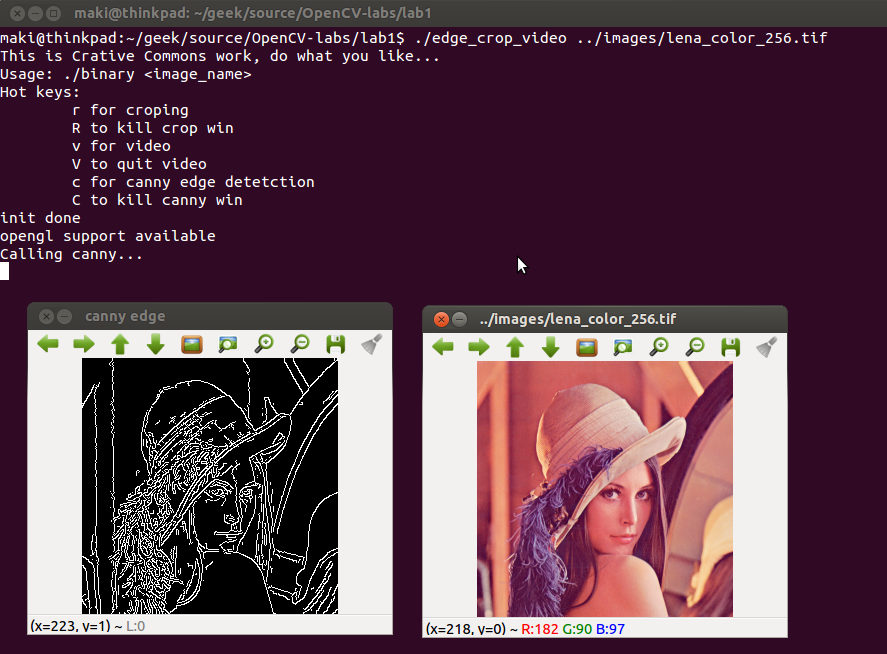
\includegraphics[scale=0.4]{images/lab1-01-edge.png}
% \caption{Detekcija rubova}
% % \label{fig:lab1-01-edge}
% \end{figure}

\newpage
\subsubsection{Rezanje slike}
Rezanje slike (engl. \textit{cropping}) je implementirano kroz poziv par
funkcija. Pritiskom na tipku \textbf{``r''} postavlja se
\textit{setMouseCallback} (funkcija koja konstantno poziva drugu
funkciju u slučaju micanja miša ili pritiska tipke) na funkciju
\textit{onMouse}. Funkciji \textit{onMouse} se također kroz
\textit{setMouseCallback} predaje i slika nad kojom je definiran
\textit{callback}.
\\

\begin{lstlisting}[language=C,caption={Rezanje slike}]
void onMouse( int event, int x, int y, int flags, void* param ) {
    Mat& image = *(Mat*) param;
    switch( event ) {
        case CV_EVENT_LBUTTONDOWN:
            drawing_box = true;
            box = Rect(x, y, 0, 0);
            break;
        case CV_EVENT_MOUSEMOVE: 
            if( drawing_box ) {
                box.width = x-box.x;
                box.height = y-box.y;
            } break;
        case CV_EVENT_LBUTTONUP: 
            drawing_box = false;
            if( box.width<0 ) {
                box.x+=box.width;
                box.width *= -1;
            }
            if( box.height<0 ) {
                box.y+=box.height;
                box.height*=-1;
            }
            draw_box( image, box );
            crop_image( image, box);
            break; } } 
void draw_box( Mat& img, Rect rect ){
    rectangle( img, rect.tl(), rect.br(), Scalar(0,0,255));
}
void crop_image( Mat& img, Rect rect ){
    Mat imgRoi = img(rect);
    namedWindow( "ImgROI", CV_WINDOW_AUTOSIZE );
    imshow( "ImgROI", imgRoi );
}
\end{lstlisting}

% \begin{figure}[h]
% \centering
% 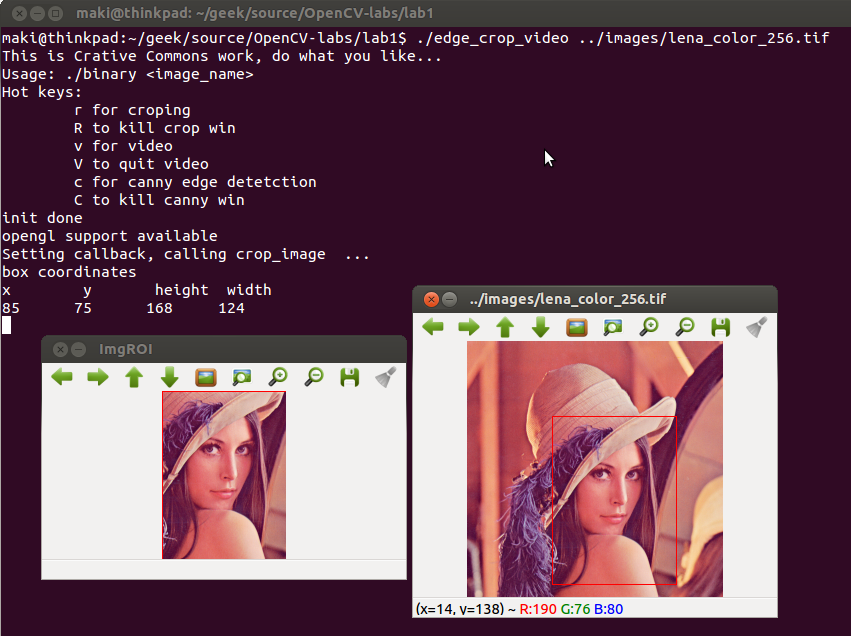
\includegraphics[scale=0.4]{images/lab1-02-crop.png}
% \caption{Rezanje slike}
% % \label{fig:lab1-02-crop}
% \end{figure}

\newpage
\subsubsection{Učitavanje videa}
Učitavanje videa ili kamere se događa nakon pritiska tipke
\textbf{``v''}. Time pozivamo funkciju \textit{init\_camera} koja
stvori objekt tipa \textit{VideoCapture}. Objekt prvo pokušu učitat
kameru ako ne uspije provjerava \textit{argv[2]} za drugim izvorom
kamere ili videa. Nakon toga u beskonačnoj petlji objekta se izvlači 
frame po frame i prikazuje u prozoru \textit{``camera``}.
\\
\begin{lstlisting}[language=C,caption={Učitavanje videa}]
void init_camera(){
    cout << "Starting camera mode... \n";
    VideoCapture cap(0);
    if( !cap.isOpened() ){
        cout << "isprobavam argv2 " 
            << global_argv[2] << endl;
        cap.open( global_argv[2] );
        if( !cap.isOpened() ){
            cerr << "fail i preko argv[2] \n"; 
            } 
        }
    while( 1 ){
        cap >> frame;
        if(!frame.data) break;
        namedWindow( "camera", CV_WINDOW_AUTOSIZE );
        imshow( "camera", frame );
        char c = waitKey(10);
        if( c == 'V' ){
            destroyWindow("camera");
            break; 
            } 
        } 
    }
\end{lstlisting}


\subsection{Zaključak}


Osnovni zadaci ove vježbe su bili upoznavanje s OpenCV bibliotekom,
podešavanje radne okoline i rješavanje par jednostavnijih zadataka.
Inicijalno podešavanje radne okoline je bitan zadatak jer o njemu ovisi
izvedba ove i budućih vježbi.
S OpenCV bibliotekom smo se upoznali kroz rješavanje zadataka.
Pisanje jednostavnog programa za detektiranje rubova na slici nam je
pružilo uvid u deklariranje \textit{Mat} varijabli za spremanje slika,
pozivanje OpenCV funkcija i prikazivanje tih slika.
Rješavanje problema rezanja slike nam je omogućilo upoznavanje s
\textit{mouseCallback} funkcijom koja je sastavni dio većine grafičkih
programa. Njeno razumjevanje je ključan dio za pisanje programa koji traže
interakciju s korisnikom. Osim toga naučili korisiti funkciju
\textit{rectangle} za crtanje pravokutnika na slici i definirati regiju
intersa na slici. 
Zadnji dio zadatka se odnosio na učitavanje videa. Osnovna stvar je bila
shvatiti kako \textit{VideoCapture} objekt funkcionira, te koje njegove
metode možemo korisiti.
Svi ovi zadaci su okosnice drugi programa. Detekcija rubova na slici s
kamere se može korisiti u programu koji detektira pokret.
Rezanje slike je poželjna funkcija svakog preglednika slika.

